\section{Aufbau und Durchführung}
\subsection{Aufbau}
Wie in Kapitel \ref{sec:1} beschrieben, wird die Lebensdauer der einzelnen Myonen bestimmt, indem die Zeitdifferenz zwischen Eintreffen
des Myons im Szintillator und dem folgenden Zerfall gemessen wird. Problematisch hierbei ist, dass die meisten Myonen eine so hohe Energie haben, dass
sie im Szintillator nicht vollständig abgebremst werden und somit nicht innerhalb des Szintillators zerfallen. Diese Myonen senden also nur ein Start-Signal,
aber kein Stopp-Signal, sodass solche Signale abgefangen werden müssen. Weiterhin zerfallen nicht alle negativen Myonen sofort, sondern manche werden zunächst von einem
Atomkern eingefangen und bilden ein myonisches Atom.

\begin{figure}[h]
  \centering
  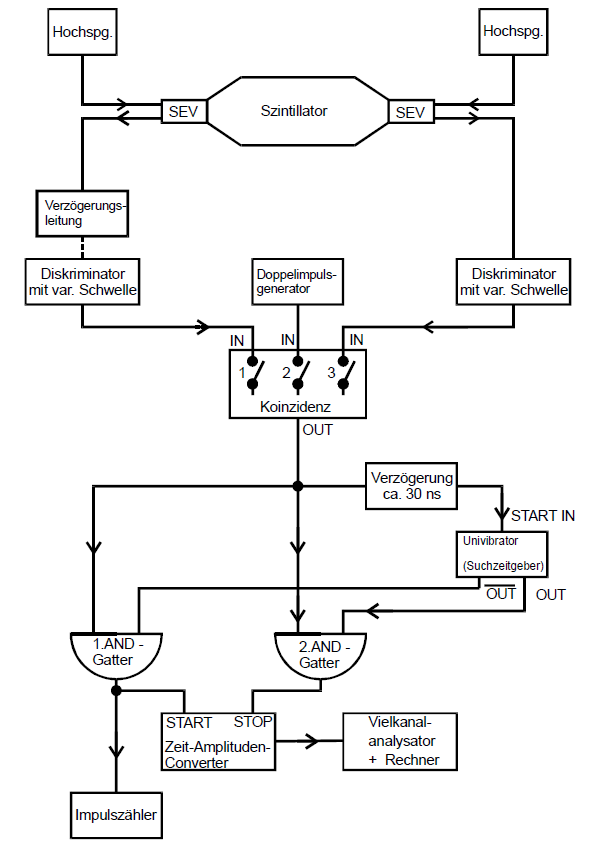
\includegraphics[scale=0.6]{graphics/aufbau.png}
  \caption{Schematischer Versuchsaufbau \cite{anleitung}.}
  \label{fig:aufbau}
\end{figure}

In Abbildung \ref{fig:aufbau} ist der verwendete Versuchsaufbau schematisch dargestellt. Aufgrund der benötigten geringen Abklingzeit wird ein organischer Szintillator
verwendet. Wie in der Abbildung deutlich wird, werden an zwei entgegengesetzten Seiten Sekundärelektronenverstärker (SEV) optisch angekoppelt. Diese wandeln die Lichtimpulse
des Szintillators in elektronische Impulse um. Ein Problem bei den SEV besteht darin, dass deren Photokathoden zu spontaner Elektronenemission neigen, welche die Messungen
verfälschen können. Deshalb werden zwei SEV verwendet und eine Koinzidenzschaltung verwendet, die nur Signale zulässt, wenn die beiden SEV innerhalb eines kurzen Intervalls "gleichzeitig"
Impulse liefern. Da die beiden SEV und deren optische Kopplung an den Szintillator leichte Unterschiede aufweisen können, wird beiden SEV jeweils eine Verzögerungsleitung nachgeschaltet, die
so angepasst wird, dass die Signale zeitgleich bei der Koinzidenzschaltung ankommen. Vor der Koinzidenzschaltung ist jeweils ein Diskriminator, der zum einen der Rauschunterdrückung dient
und zum anderen die Signale der SEV auf eine einheitliche Länge und Breite bringt, da die restliche Schaltung aus logischen Bauteilen besteht, welche dem NIM-Standard folgen.

Da die mittlere Lebensdauer der Myonen kleiner als der mittlere zeitliche Abstand zwischen zwei einfallenden Myonen ist, kann gemessen werden, indem der Impuls eines einfallenden Myons eine
Stoppuhr startet und der Impuls des zerfallenden Myons die Uhr stoppt. Dazu wird ein Zeit-Amplituden-Converter (TAC) verwendet, der einen Spannungsimpuls abgibt, dessen Amplitude proportional
zur Zeitdifferenz zwischen Start- und Stoppsignal ist. Außerdem werden die Start- und Stoppimpulse, die den TAC erreichen, von Impulszählern aufgezeichnet. Die Impulse des TAC werden von einem
Vielkanalanalysator entsprechend ihrer Höhe in 512 Kanälen histogrammiert. Zur Kalibrierung der Kanäle kann an die Koinzidenzschaltung ein Doppelimpulsgenerator angeschlossen werden, welcher
elektrische Impulse mit einer einstellbaren Zeitdifferenz erzeugen kann.

Zu berücksichtigen ist jedoch, dass die meisten Myonen zu hochenergetisch sind, sodass sie durch den Szintillator durchgehen und nicht darin komplett abgebremst werden. Dadurch geben diese
nur einen Startimpuls und keinen Stoppimpuls. Es wird also eine logische Schaltung mithilfe eines Univibrators und zweier AND-Gatter aufgebaut, die die Schaltung nach einer einstellbaren
Suchzeit $T_\text{S}$ wieder in ihren Ausgangszustand versetzt, sodass nach Ablauf dieser Zeit das nächste Signal wieder als Startsignal gewertet wird. Da die Signale der Koinzidenzschaltung
eine Länge von ca. $\SI{20}{ns}$ haben, ist vor dem Univibrator eine Verzögerungsleitung mit einer Verzögerung von ca. $\SI{30}{ns}$ eingebaut.

\subsection{Durchführung}
Zunächst muss die Schaltung aufgebaut werden und die einzelnen Komponenten müssen eingestellt werden. Angefangen wird bei den Diskriminatorschwellen, die so eingestellt werden, dass
beide Diskriminatoren die gleiche Impulsrate liefern, welche zwischen 20 und 40 Impulsen pro Sekunde liefen sollte. Dann werden die Verzögerungsleitungen so aufeinander eingestellt, dass
die maximale Anzahl an Impulsen von der Koinzidenzschaltung ausgegeben werden. Danach wird ein Oszilloskop an den Ausgang des Univibrators angeschlossen, um die Suchzeit $T_\text{S}$ einzustellen.
Gewählt wird eine Suchzeit von $\SI{20}{\micro\second}$. Nun wird die Schaltung bis zum TAC aufgebaut und dessen Funktionsweise überprüft. Dazu wird der Doppelimpulsgenerator anstelle der SEV an die
Koinzidenzschaltung angeschlossen. Der Messbereich des TACs wird an die Suchzeit $T_\text{S}$ angepasst. Zuletzt wird der Vielkanalanalysator angeschlossen und kalibriert. Dazu werden mit dem Doppelimpulsgenerator
Impulse mit verschiedenen Zeitdifferenzen erzeugt und überprüft, welche Kanäle diesen Zeitdifferenzen entsprechen. Daraus kann eine Ausgleichsgerade für den Zusammenhang zwischen Kanalnummer und Zeitdifferenz berechnet
werden.

Nach dem Aufbau der Schaltung und der Kalibrierung wird das Messprogramm gestartet und zeitgleich werden die Impulszähler gestartet. Über einen Zeitraum von $\SI{162391}{\second}$ werden Daten aufgenommen.
